\clearpage
\section{Data control region plots}
\label{sec:data-control-region-plots}

Monte Carlo simulation is being used in this analysis both in order to train the \glspl{bdt}, and in order to gain understanding on the standard model processes composition of the background. It is useful therefore to look at data compared to simulation plots in order to verify that the simulation does not diverge from the data in a significant way. However, in order not to unblind the data in sensitive regions, the comparison plots are done in a \gls{cr}. A straightforward \gls{cr} is the same as the normalization region for the background estimation methods of $\text{BDT} < 0$. The most sensitive category is chosen for this study, namely, the dimuon category. The tracker phase 1 data taking period is shown in this section, since it is comprised of higher luminosity and is expected to suffer from some data taking quality issues which are further addressed in Section~\ref{sec:data-quality}. The simulation has been normalized for phase 1 luminosity and the comparison plots can be seen in Figure~\ref{fig:data-control-plots-dimuon-phase1}. Good agreement between data and simulation can be observed in the ratio panel.


\begin{figure}[!htb]
\centering
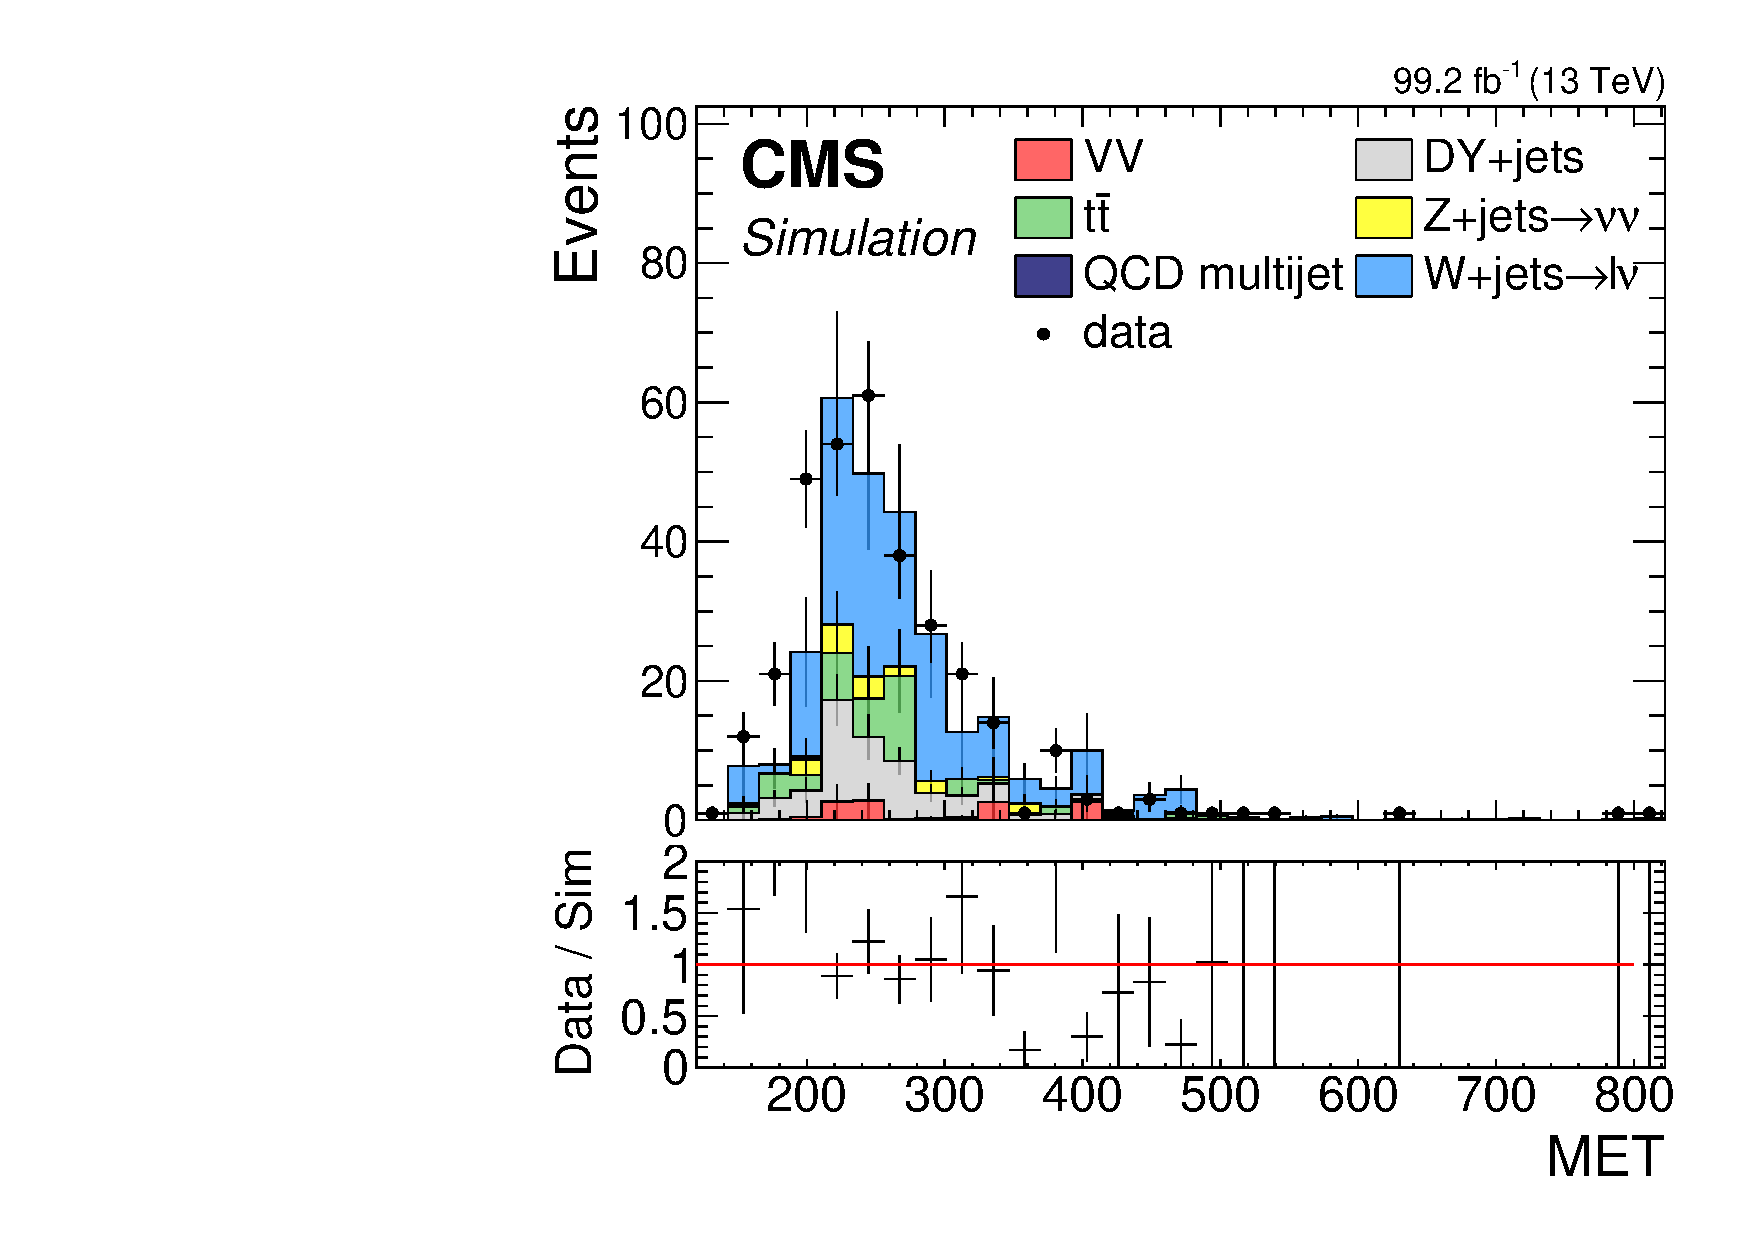
\includegraphics[width=0.48\linewidth]{plots/dilepton_muons_data_control_region_phase1/none_MET.pdf} \,
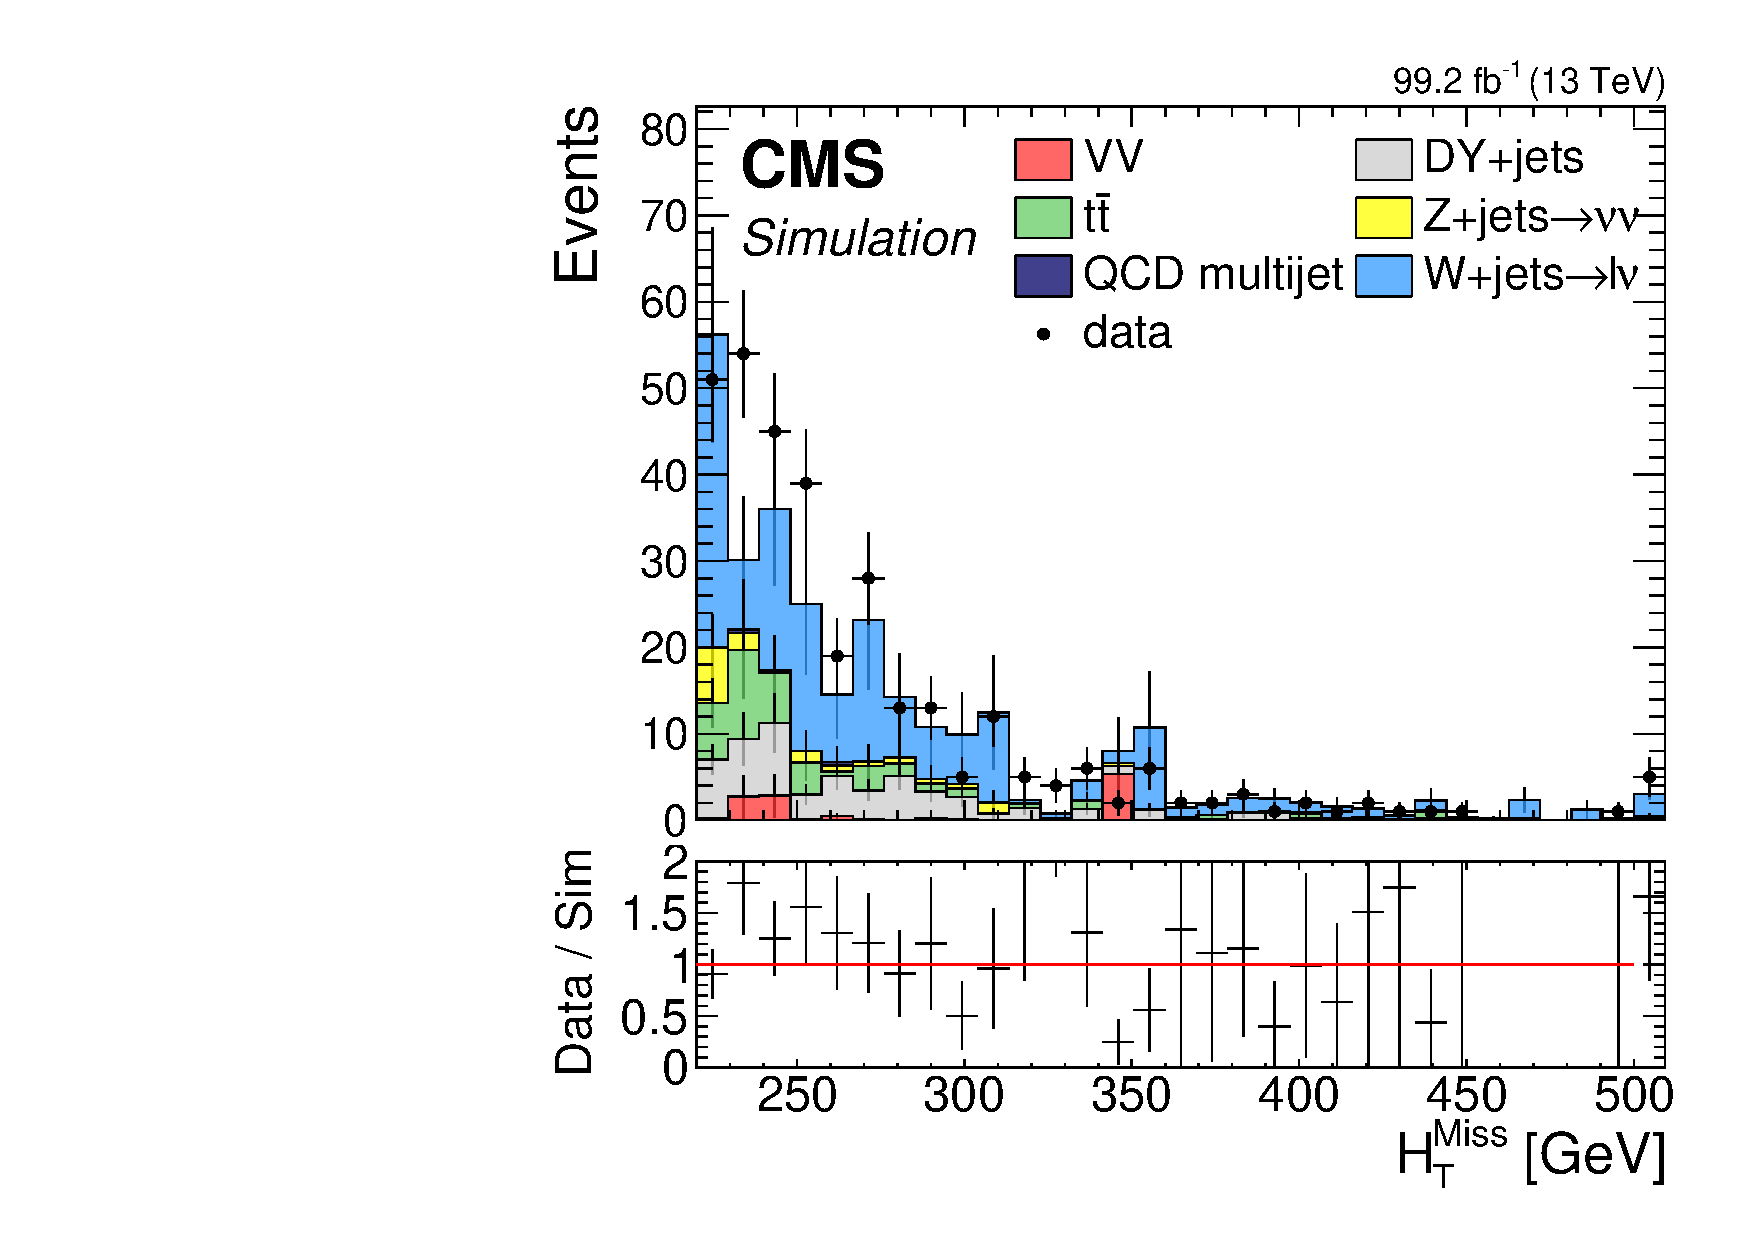
\includegraphics[width=0.48\linewidth]{plots/dilepton_muons_data_control_region_phase1/none_MHT.pdf} \\

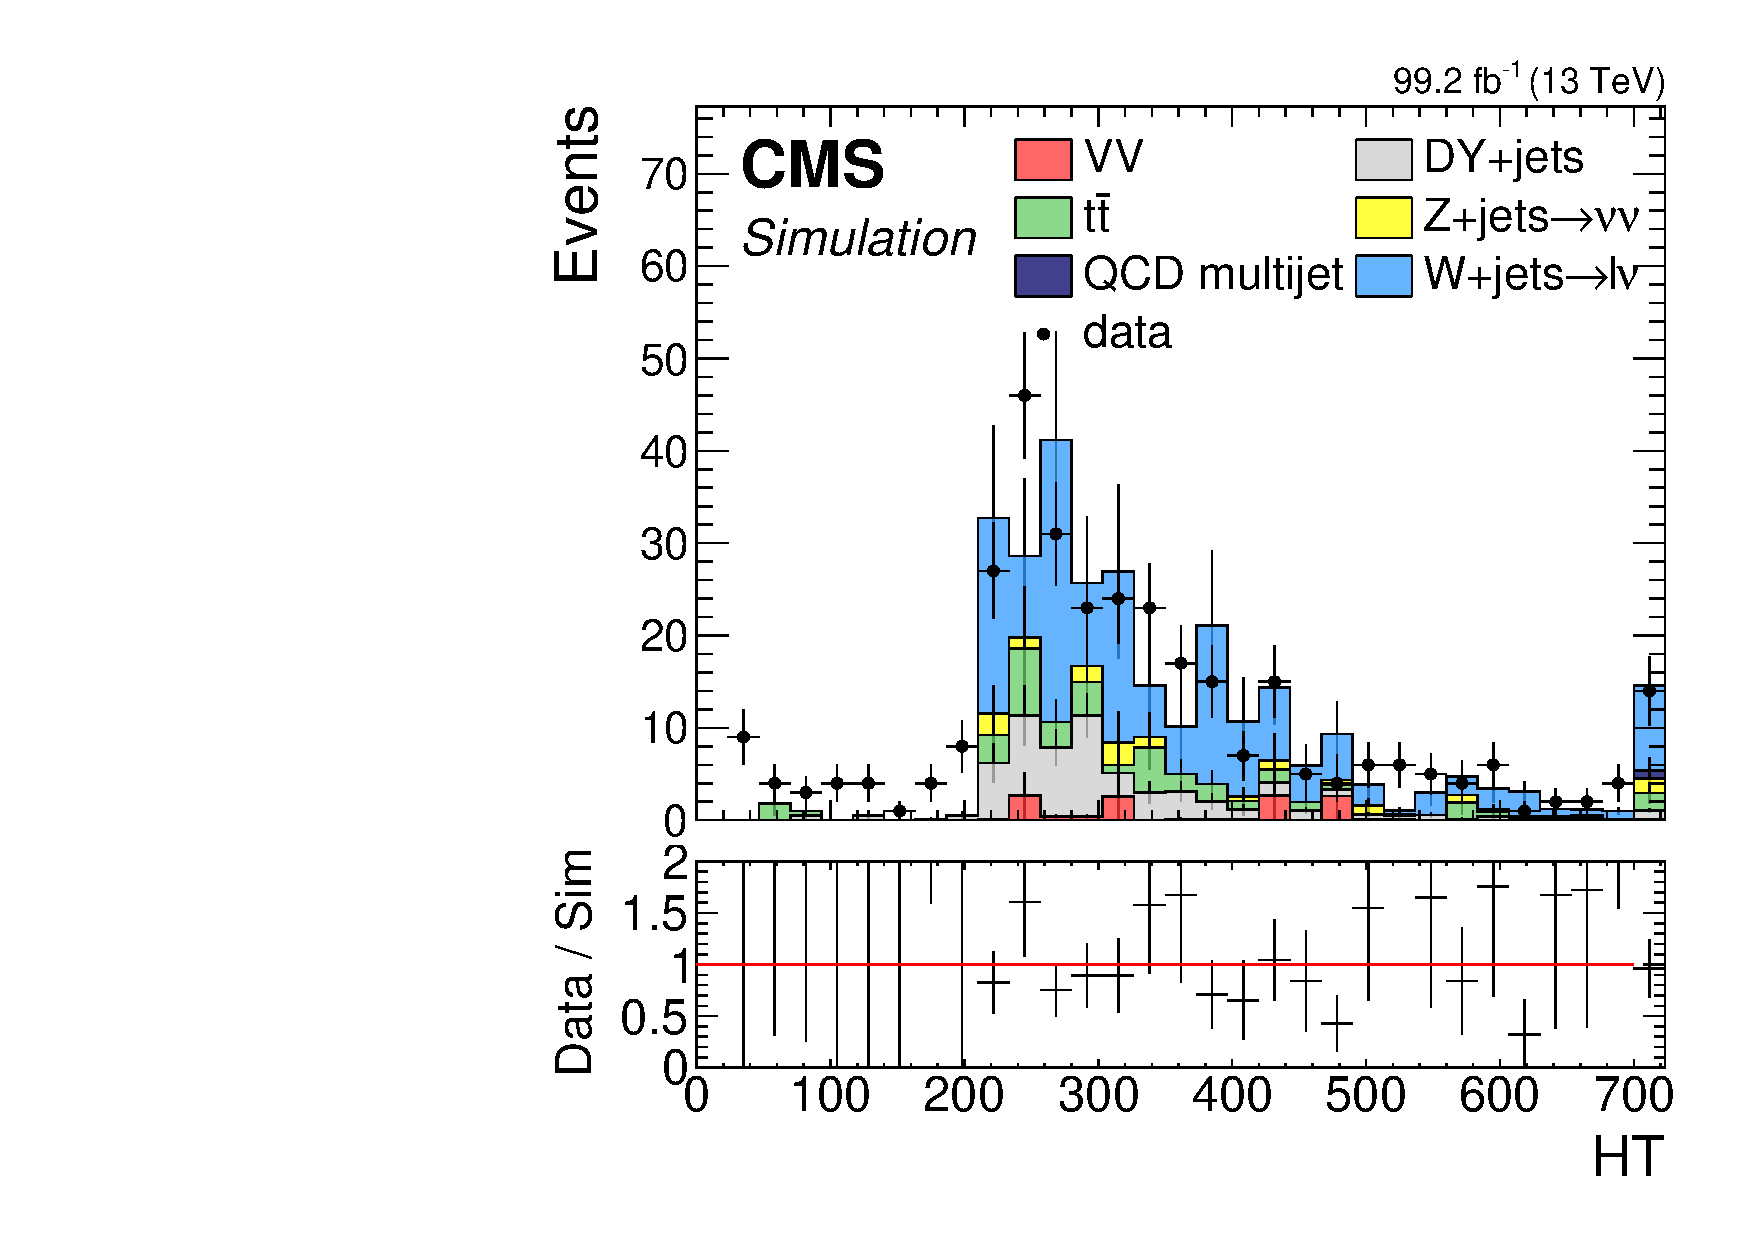
\includegraphics[width=0.48\linewidth]{plots/dilepton_muons_data_control_region_phase1/none_HT.pdf} \,
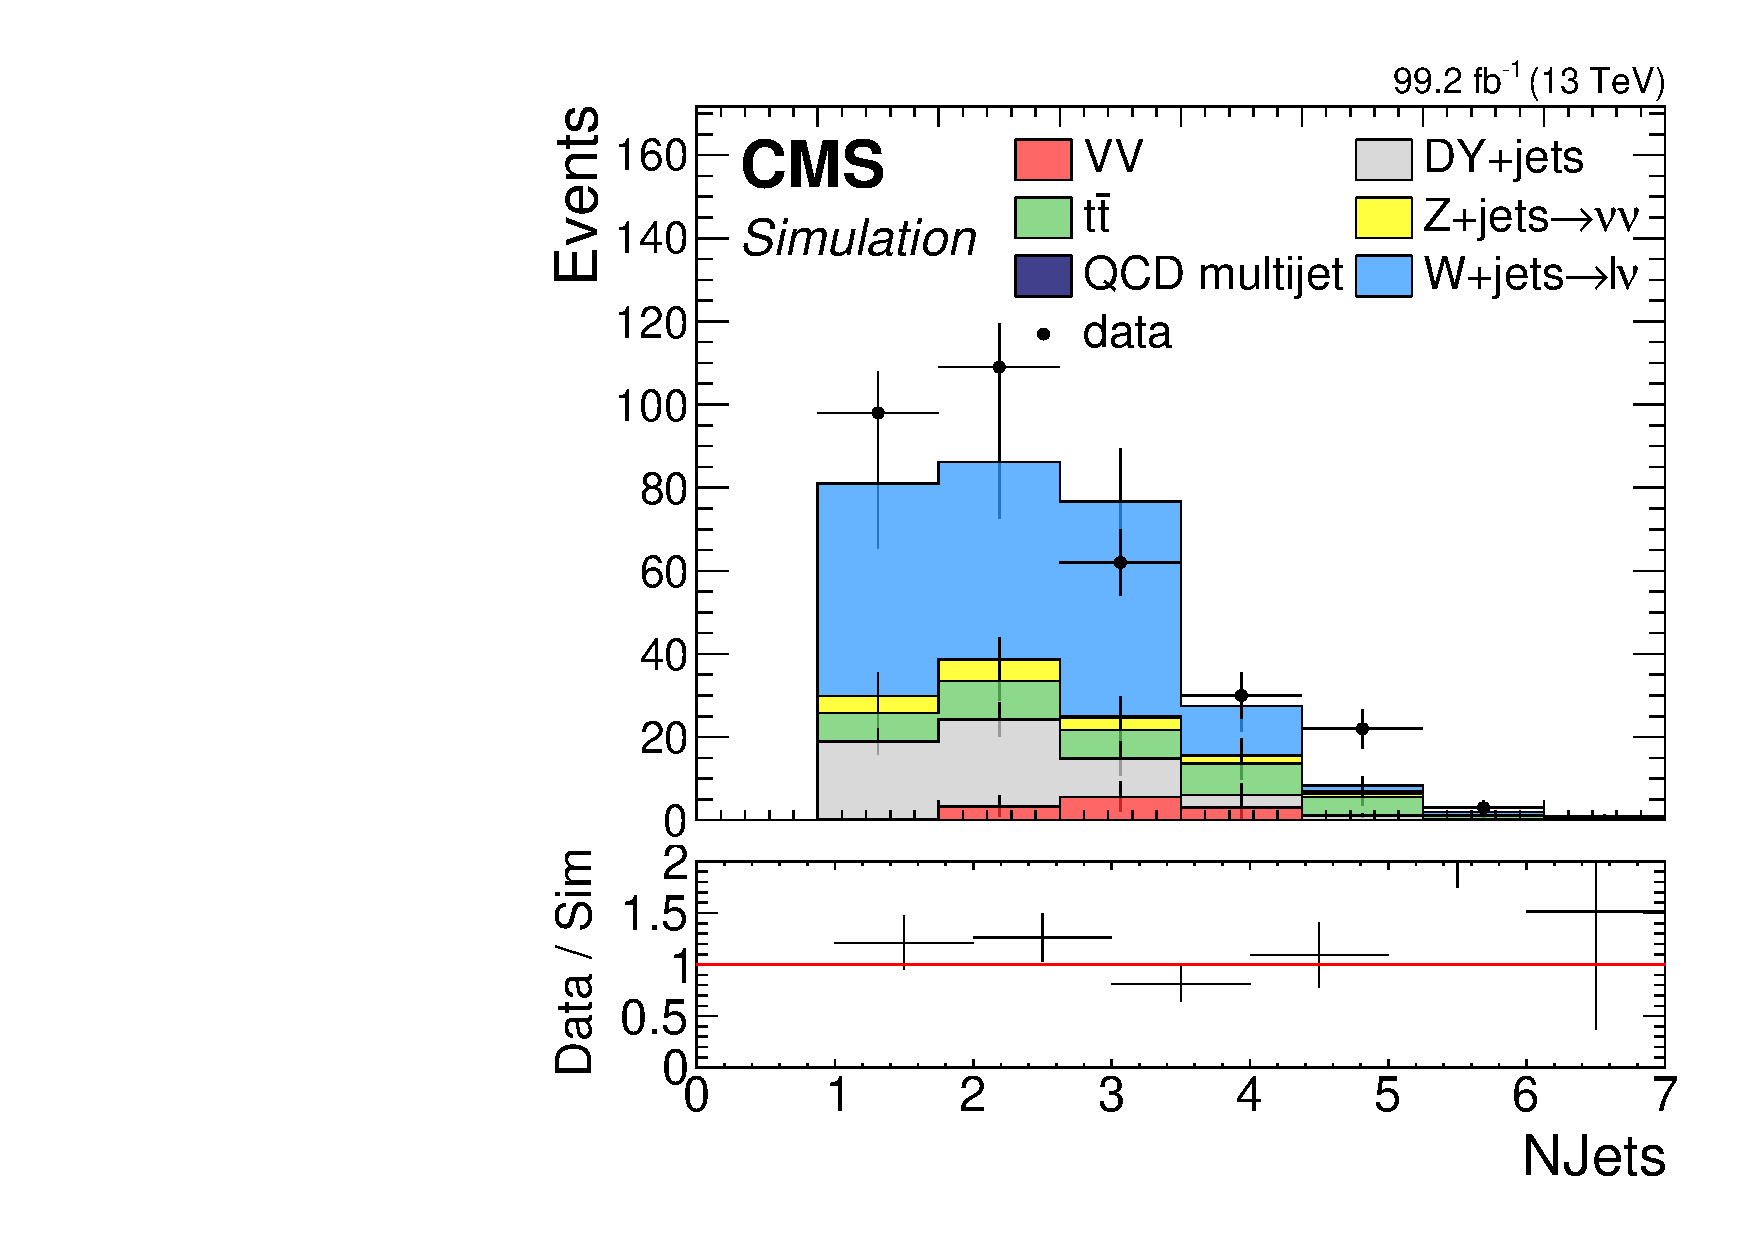
\includegraphics[width=0.48\linewidth]{plots/dilepton_muons_data_control_region_phase1/none_NJets.pdf} \\

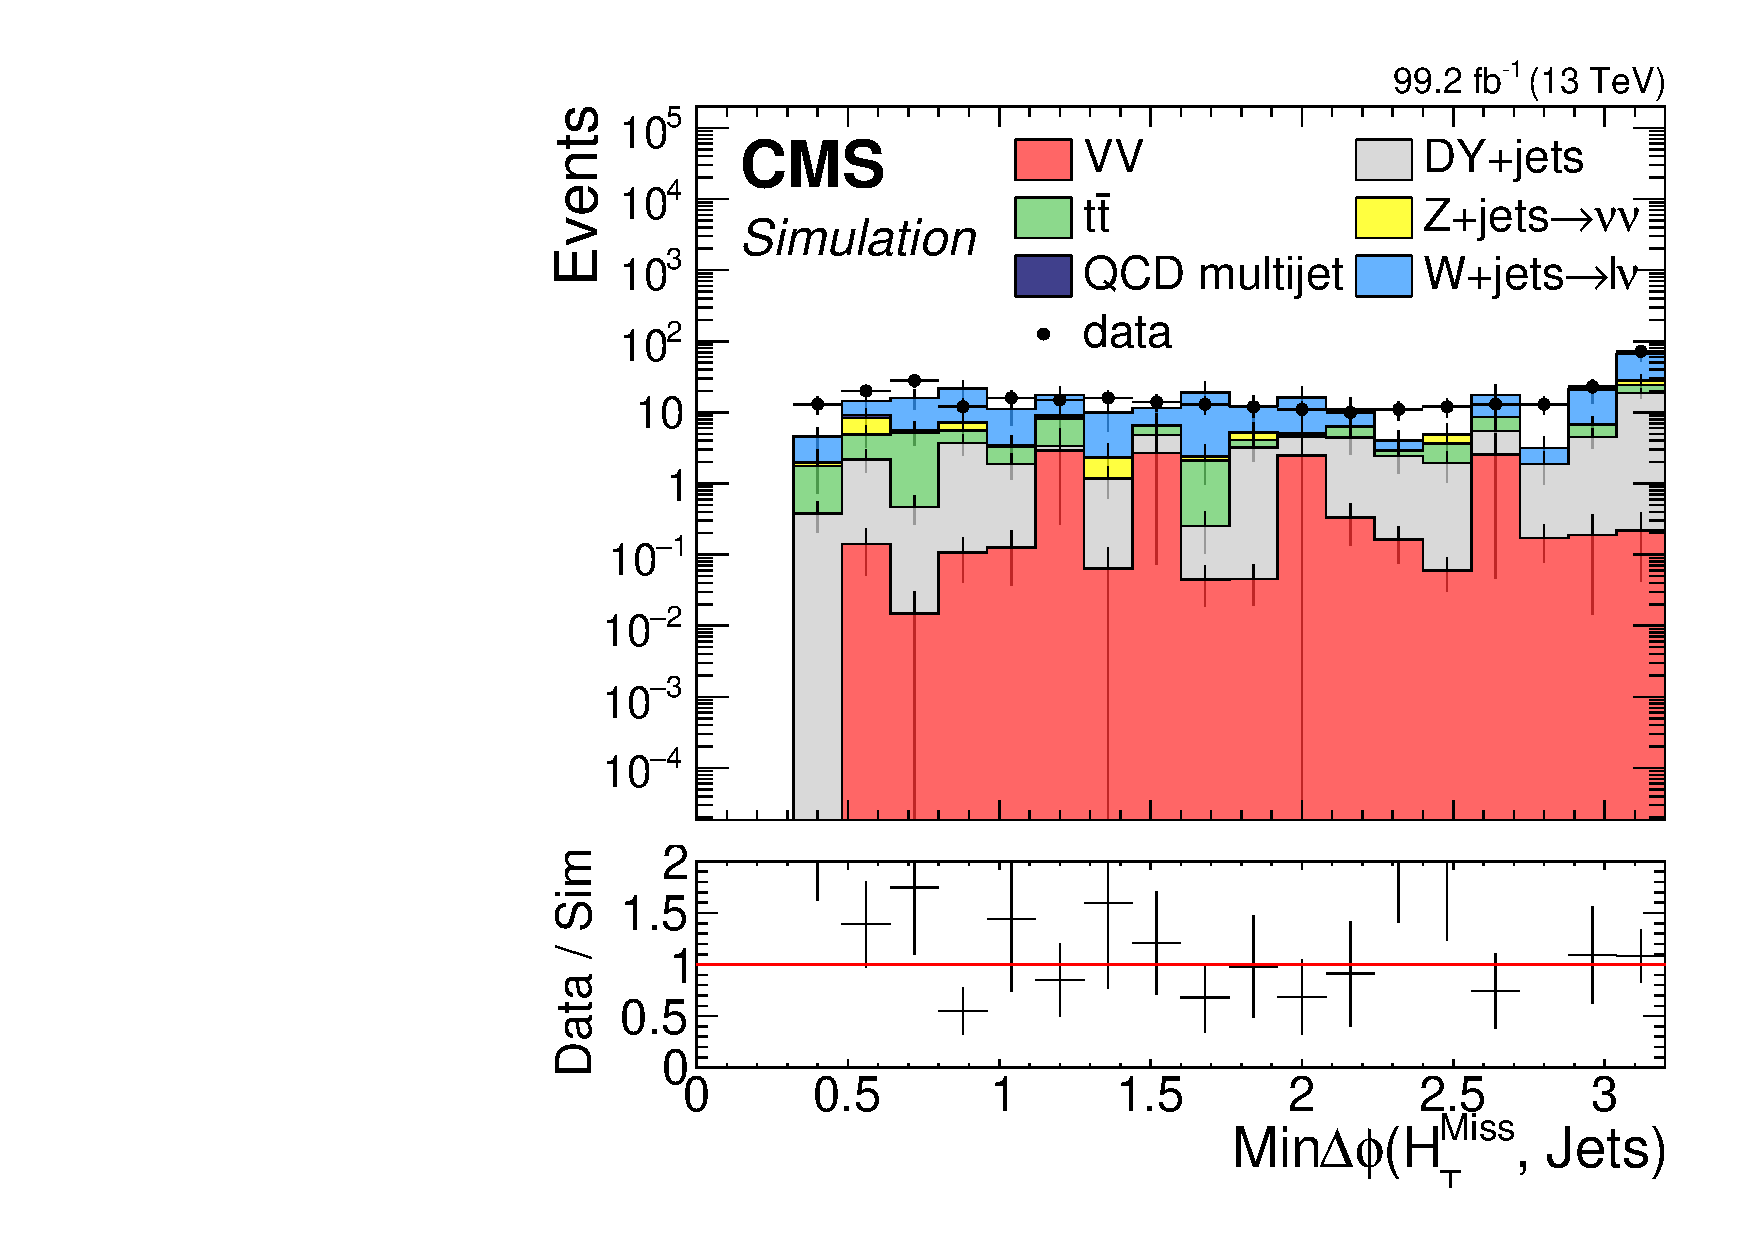
\includegraphics[width=0.48\linewidth]{plots/dilepton_muons_data_control_region_phase1/none_MinDeltaPhiMhtJets_log.pdf} \,
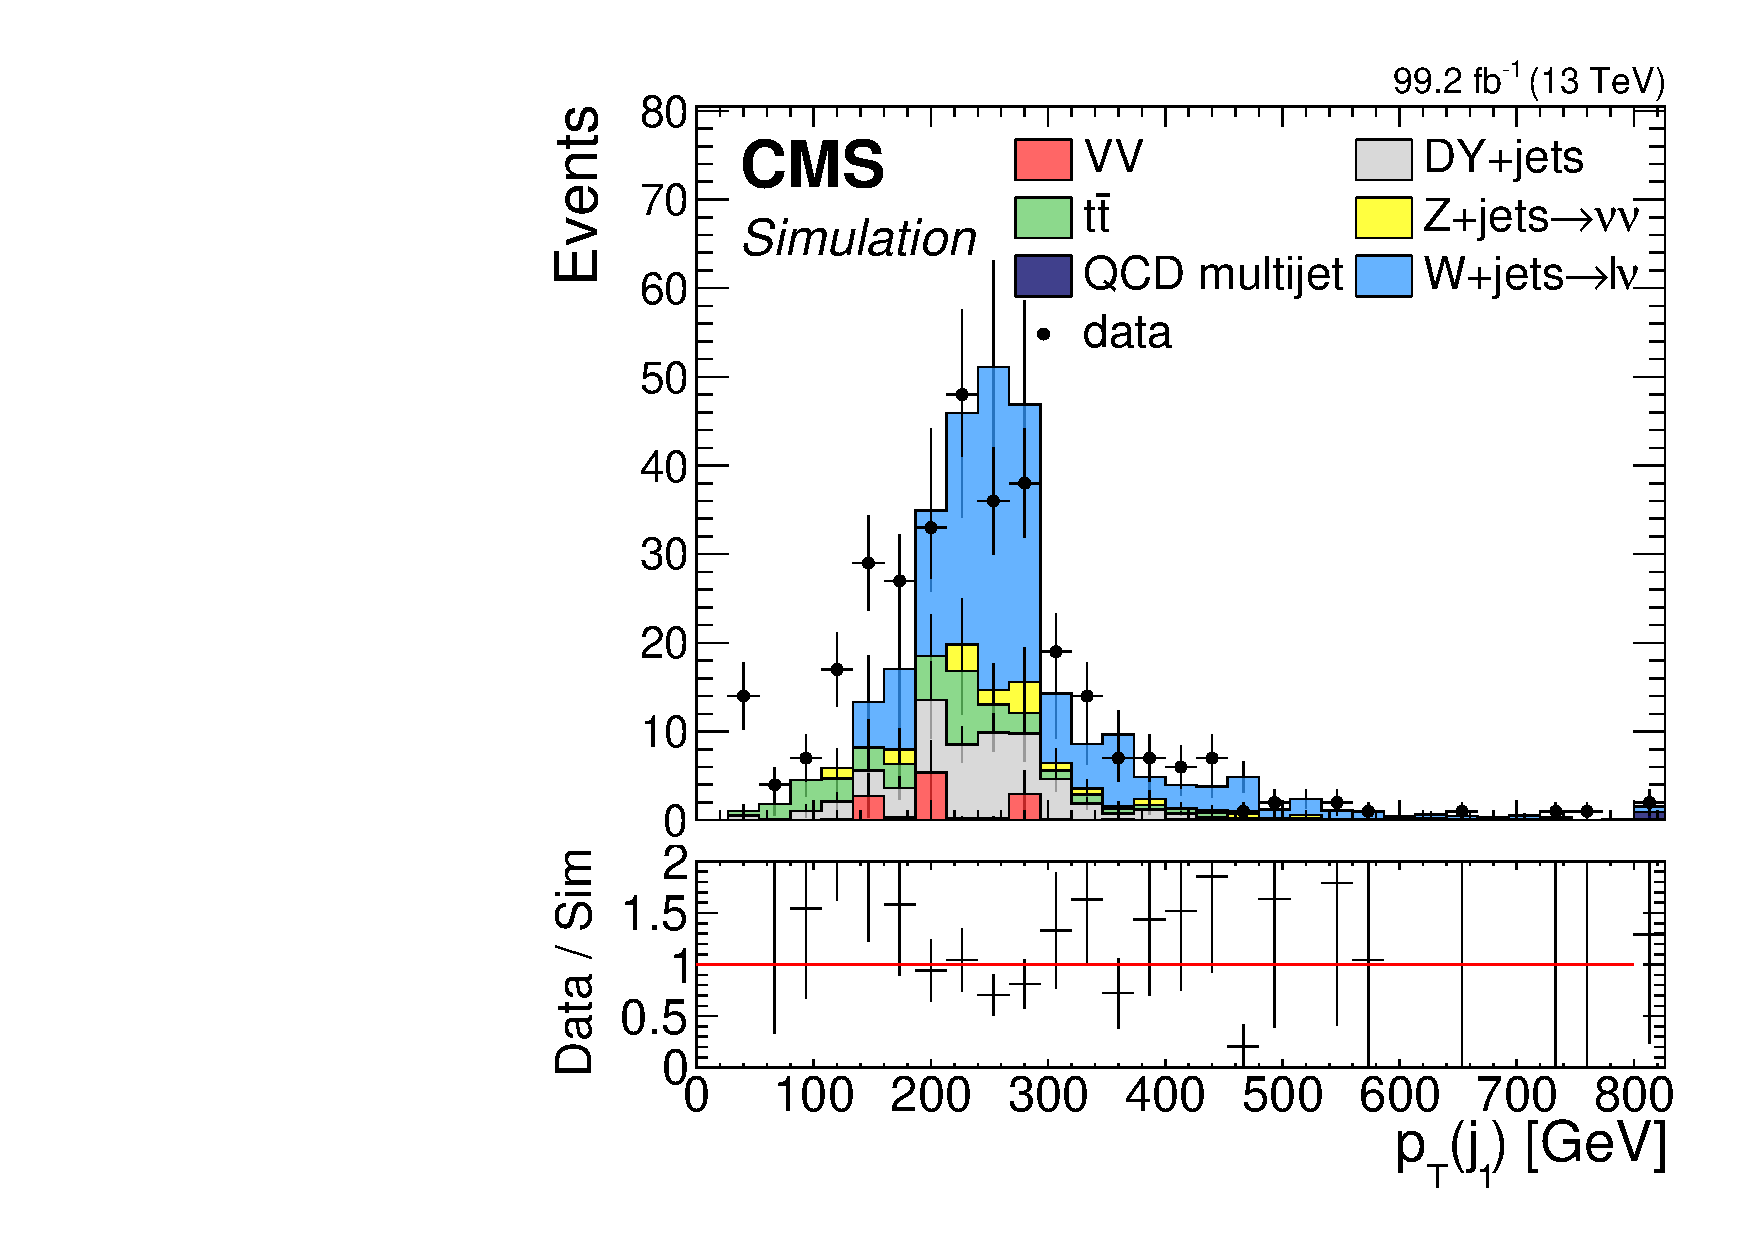
\includegraphics[width=0.48\linewidth]{plots/dilepton_muons_data_control_region_phase1/none_LeadingJetPt.pdf} \\

\caption[Data control region plots for dimuon category in phase 1]{Data control region plots for dimuon category in phase 1.}
\label{fig:data-control-plots-dimuon-phase1}
\end{figure} 


\begin{figure}[!htb]
\centering
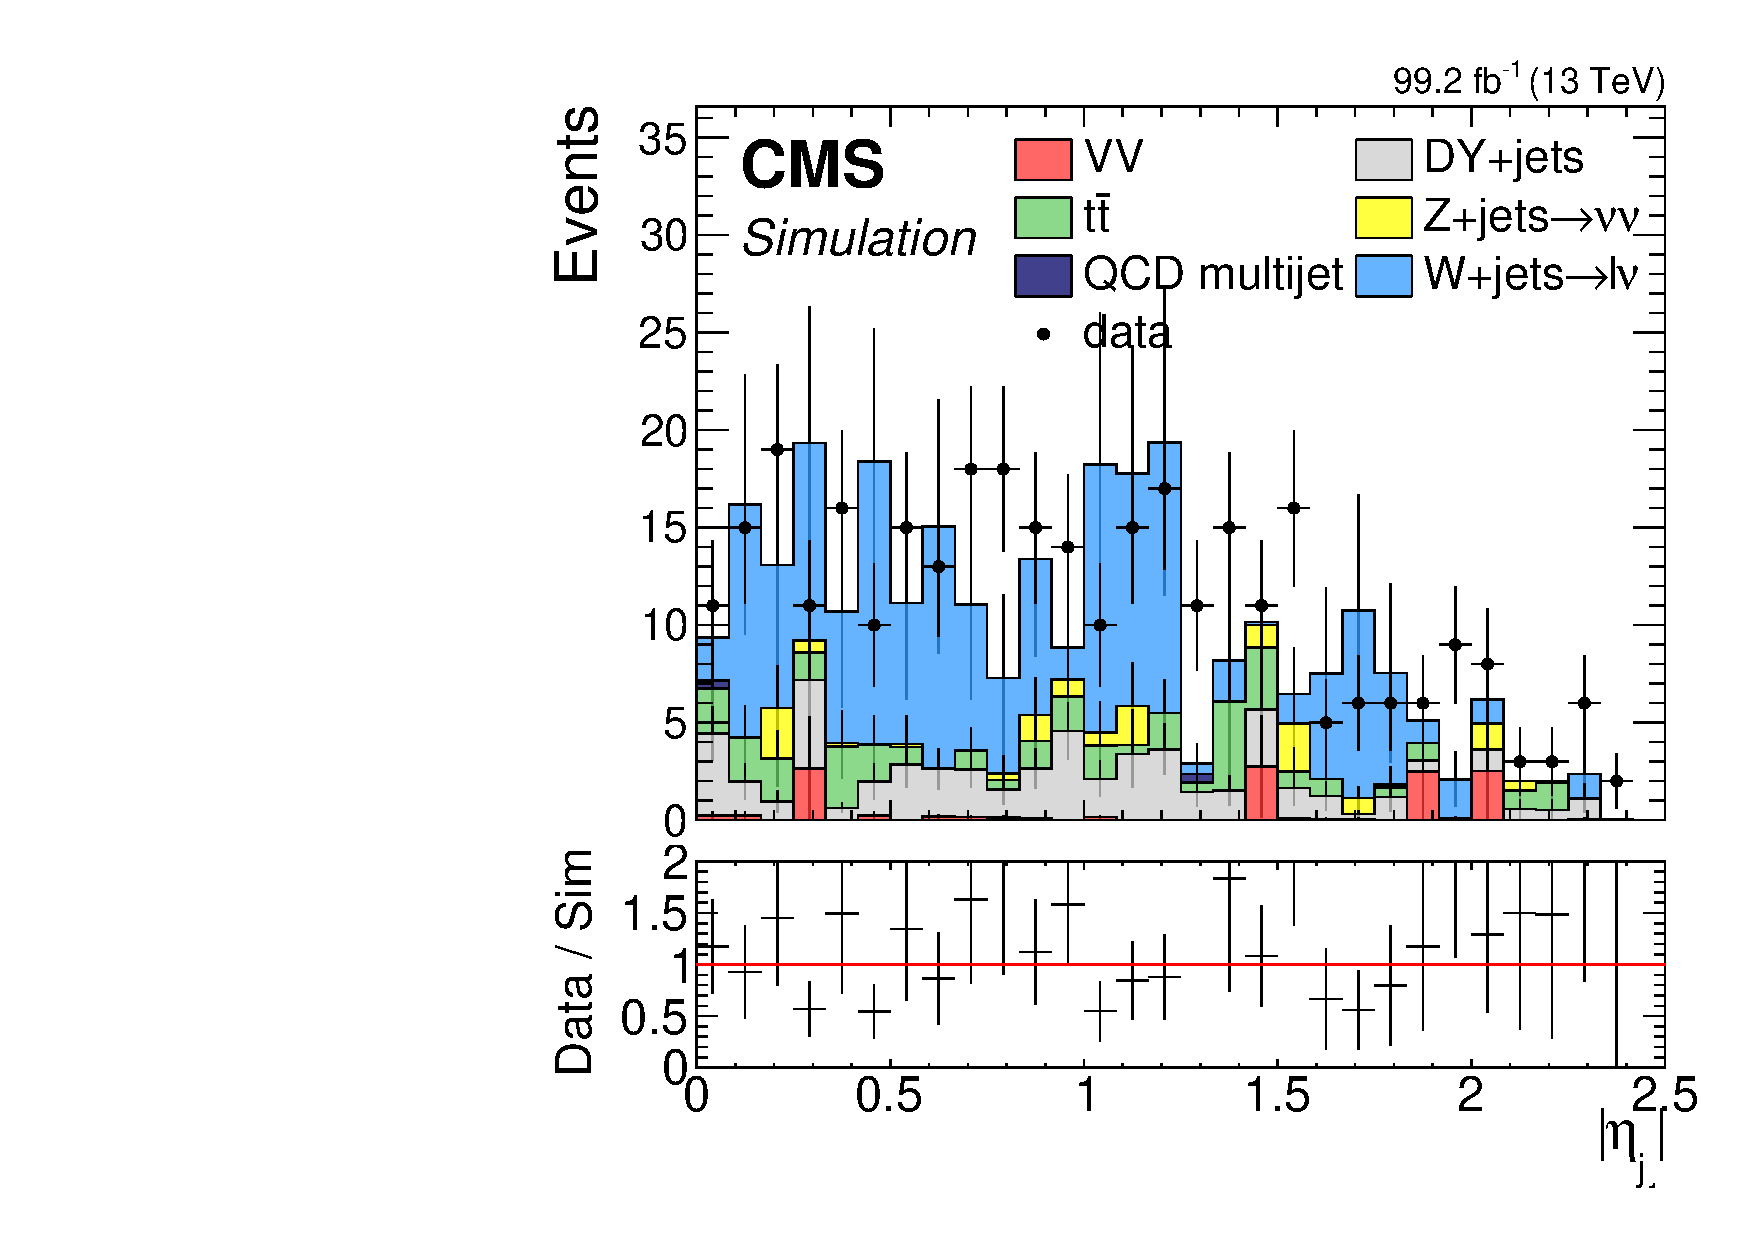
\includegraphics[width=0.48\linewidth]{plots/dilepton_muons_data_control_region_phase1/none_abs(LeadingJet.Eta()).pdf} \,
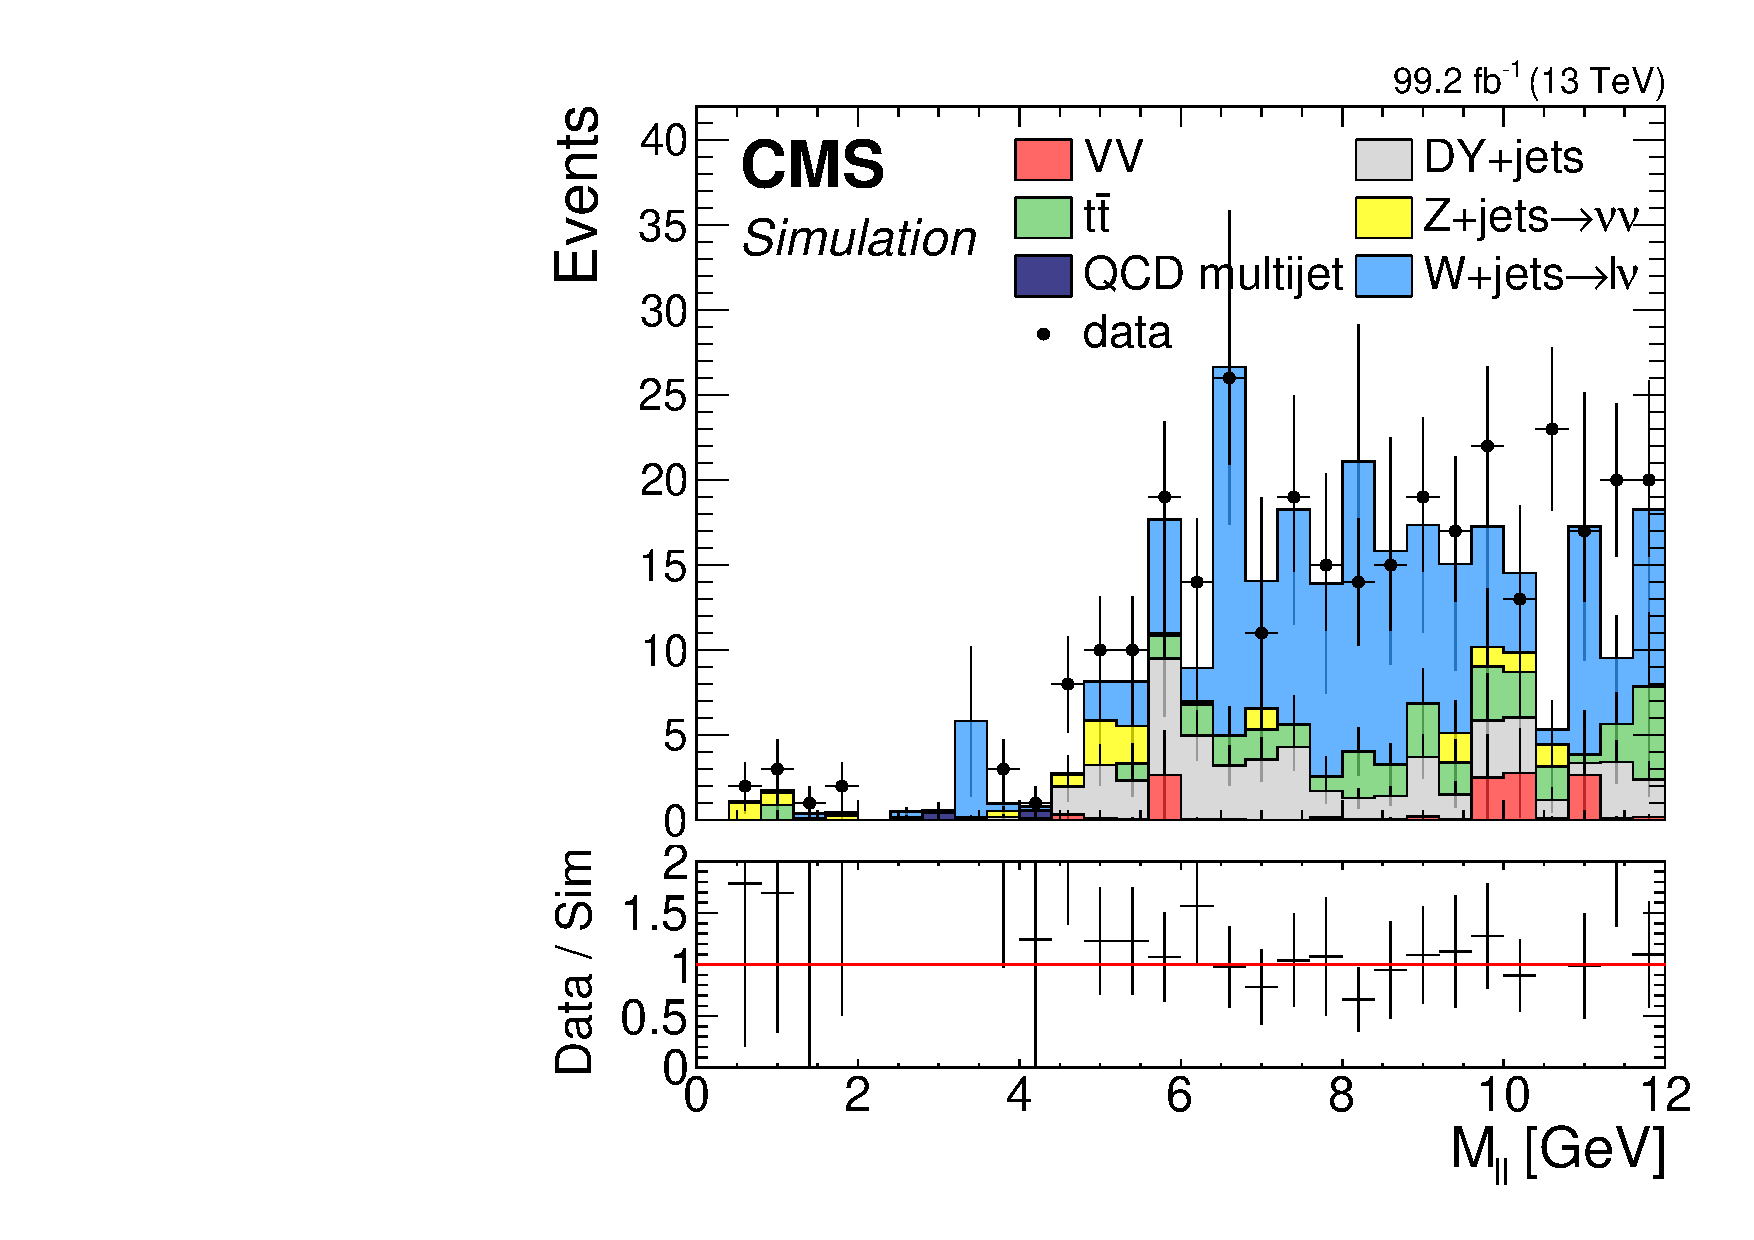
\includegraphics[width=0.48\linewidth]{plots/dilepton_muons_data_control_region_phase1/none_invMassCorrJetNoMultIso10Dr0.6.pdf} \\

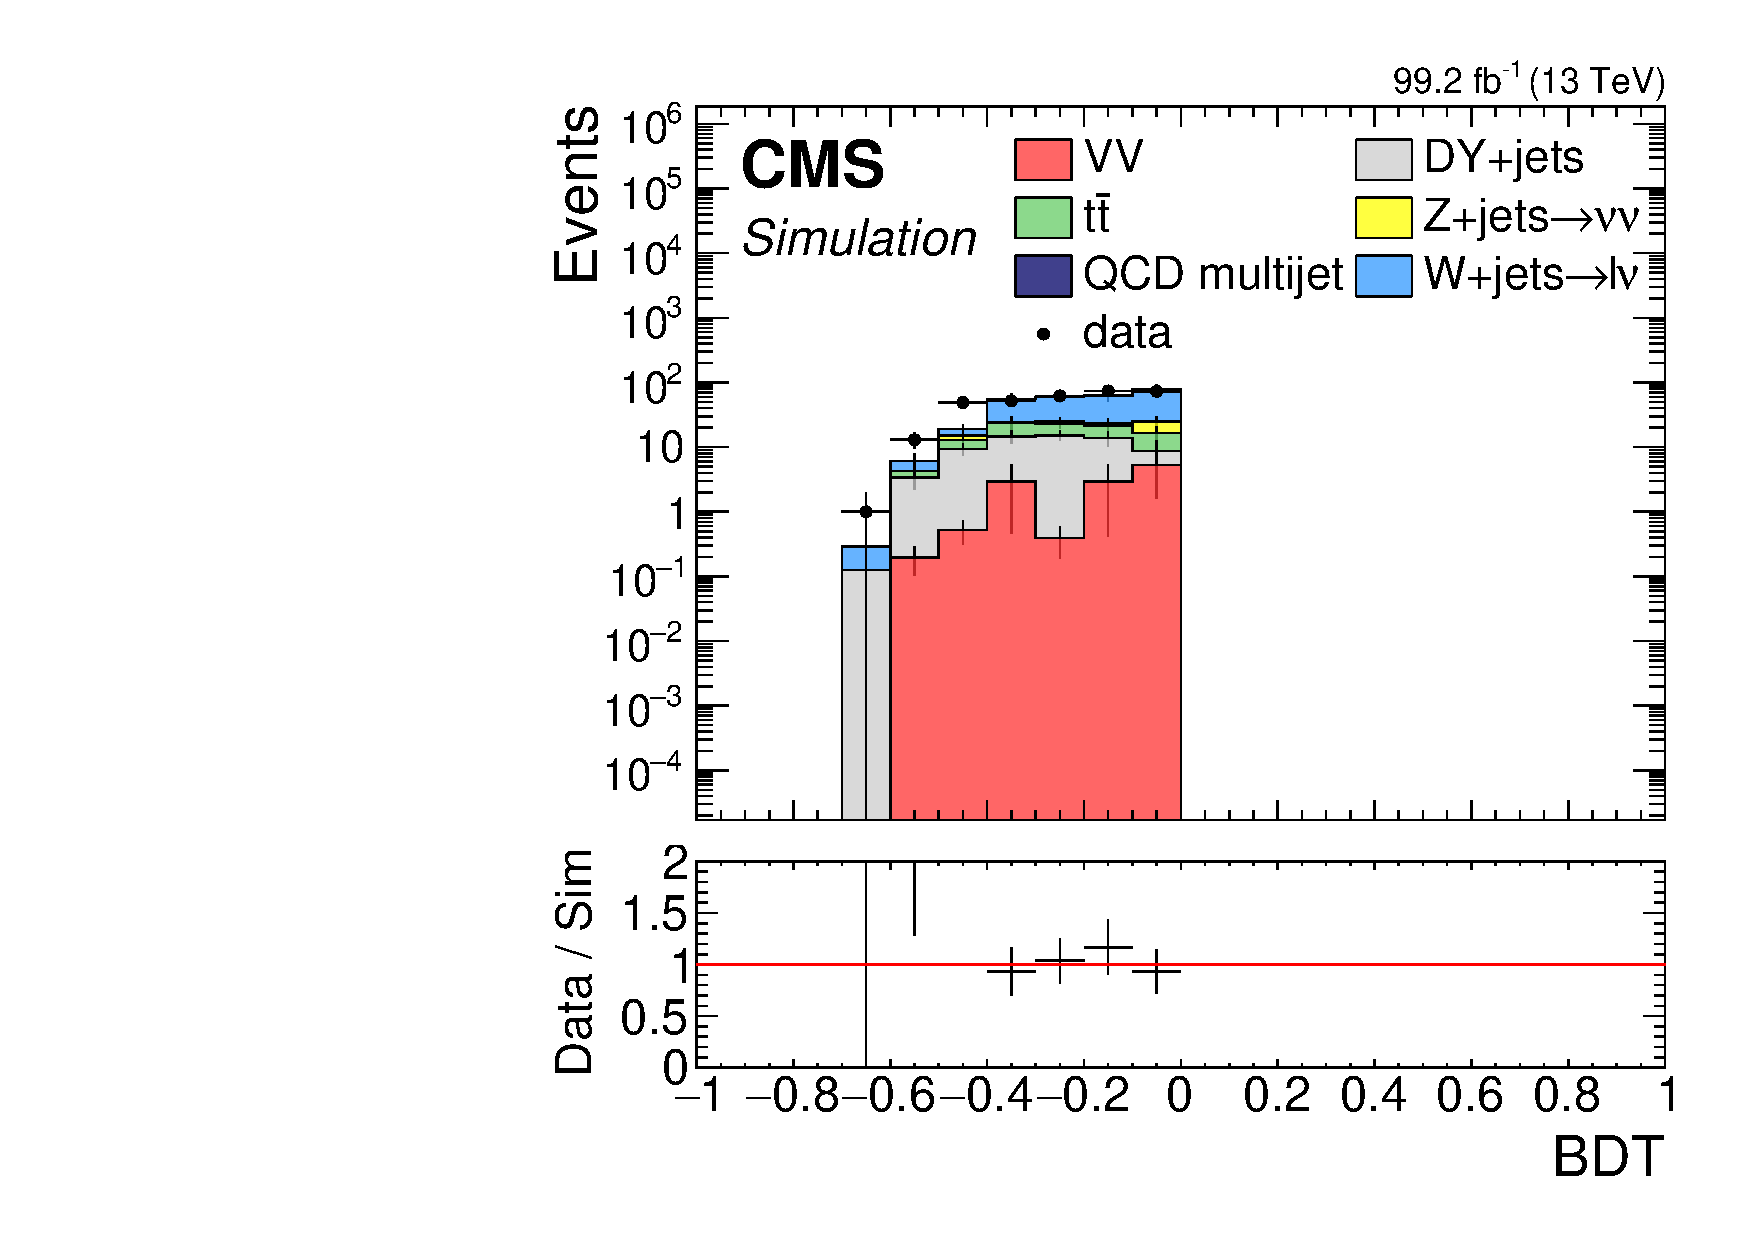
\includegraphics[width=0.48\linewidth]{plots/dilepton_muons_data_control_region_phase1/none_custom_dilepBDTCorrJetNoMultIso10Dr0.6_log.pdf} \,
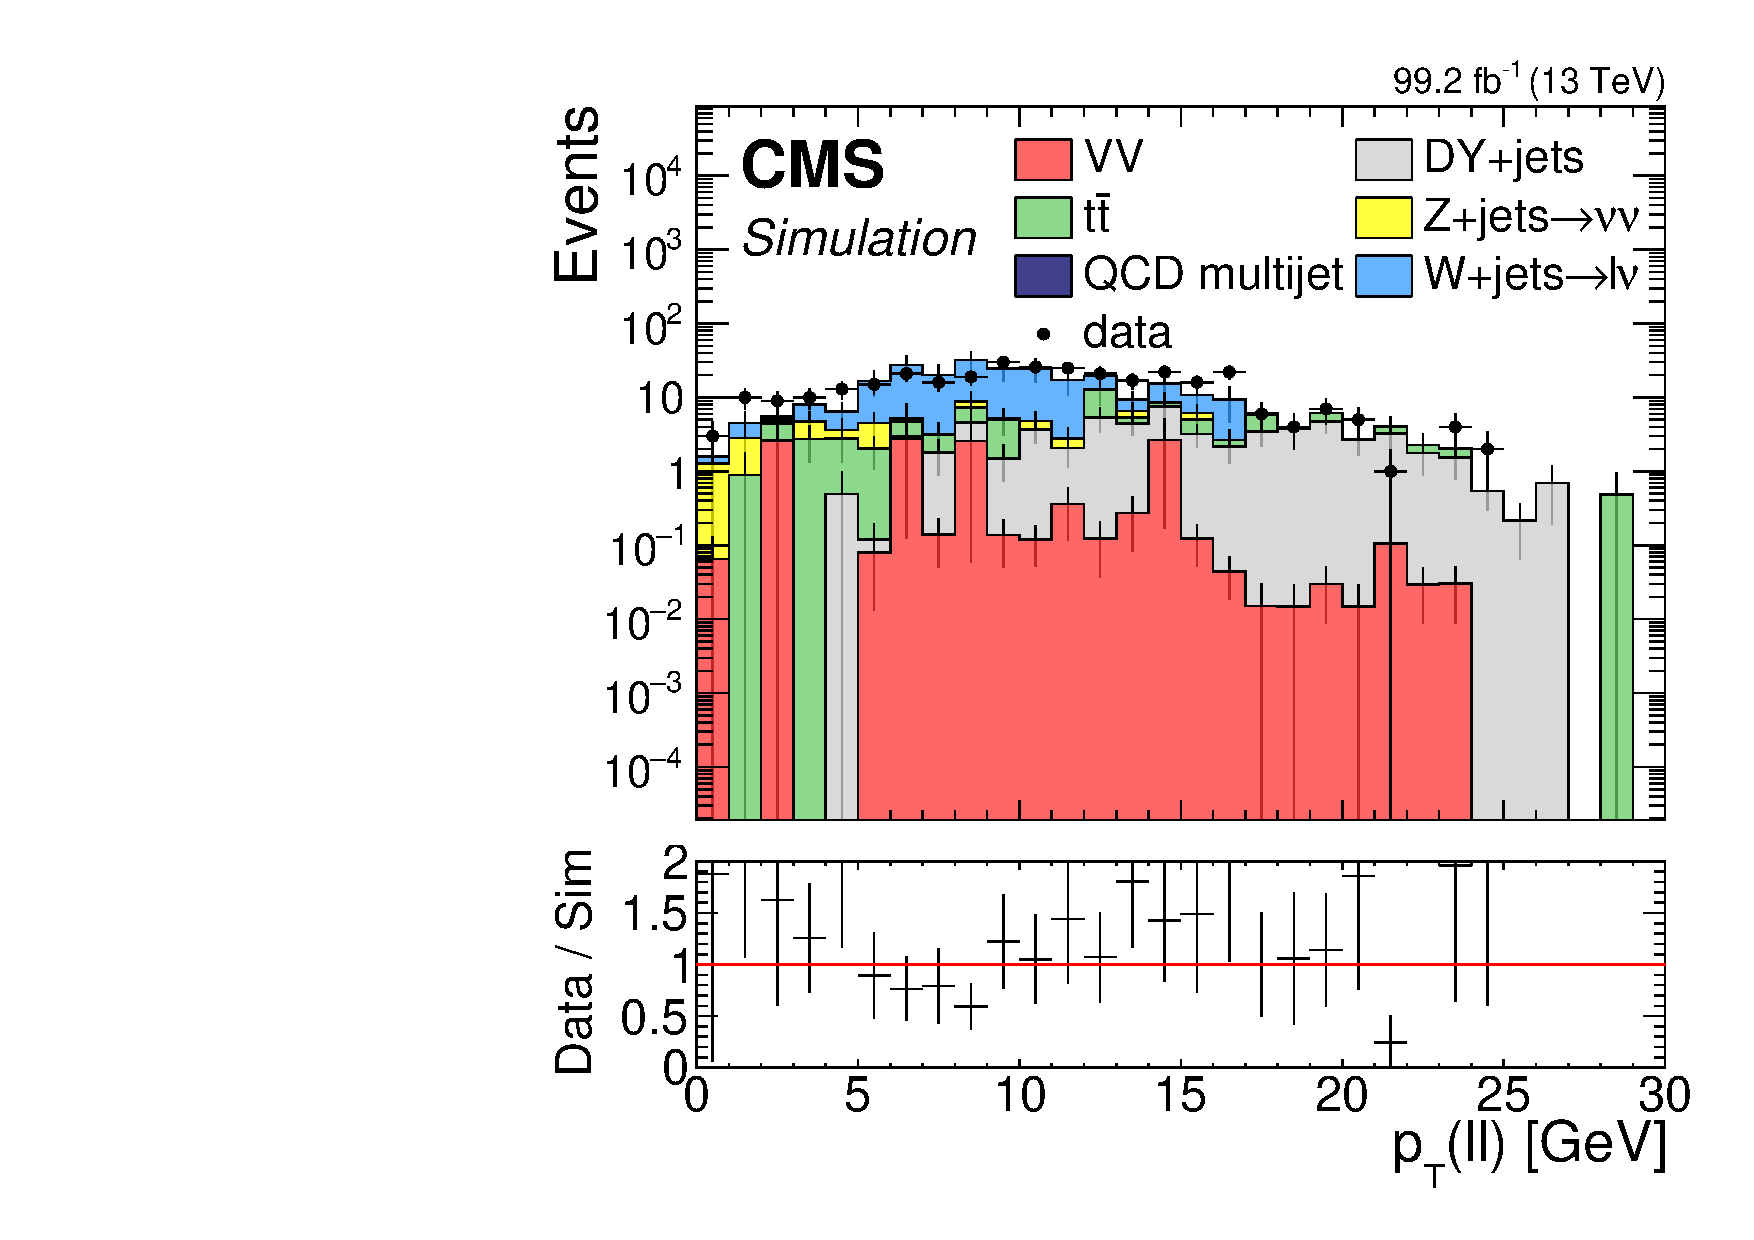
\includegraphics[width=0.48\linewidth]{plots/dilepton_muons_data_control_region_phase1/none_dileptonPtCorrJetNoMultIso10Dr0.6_log.pdf} \\

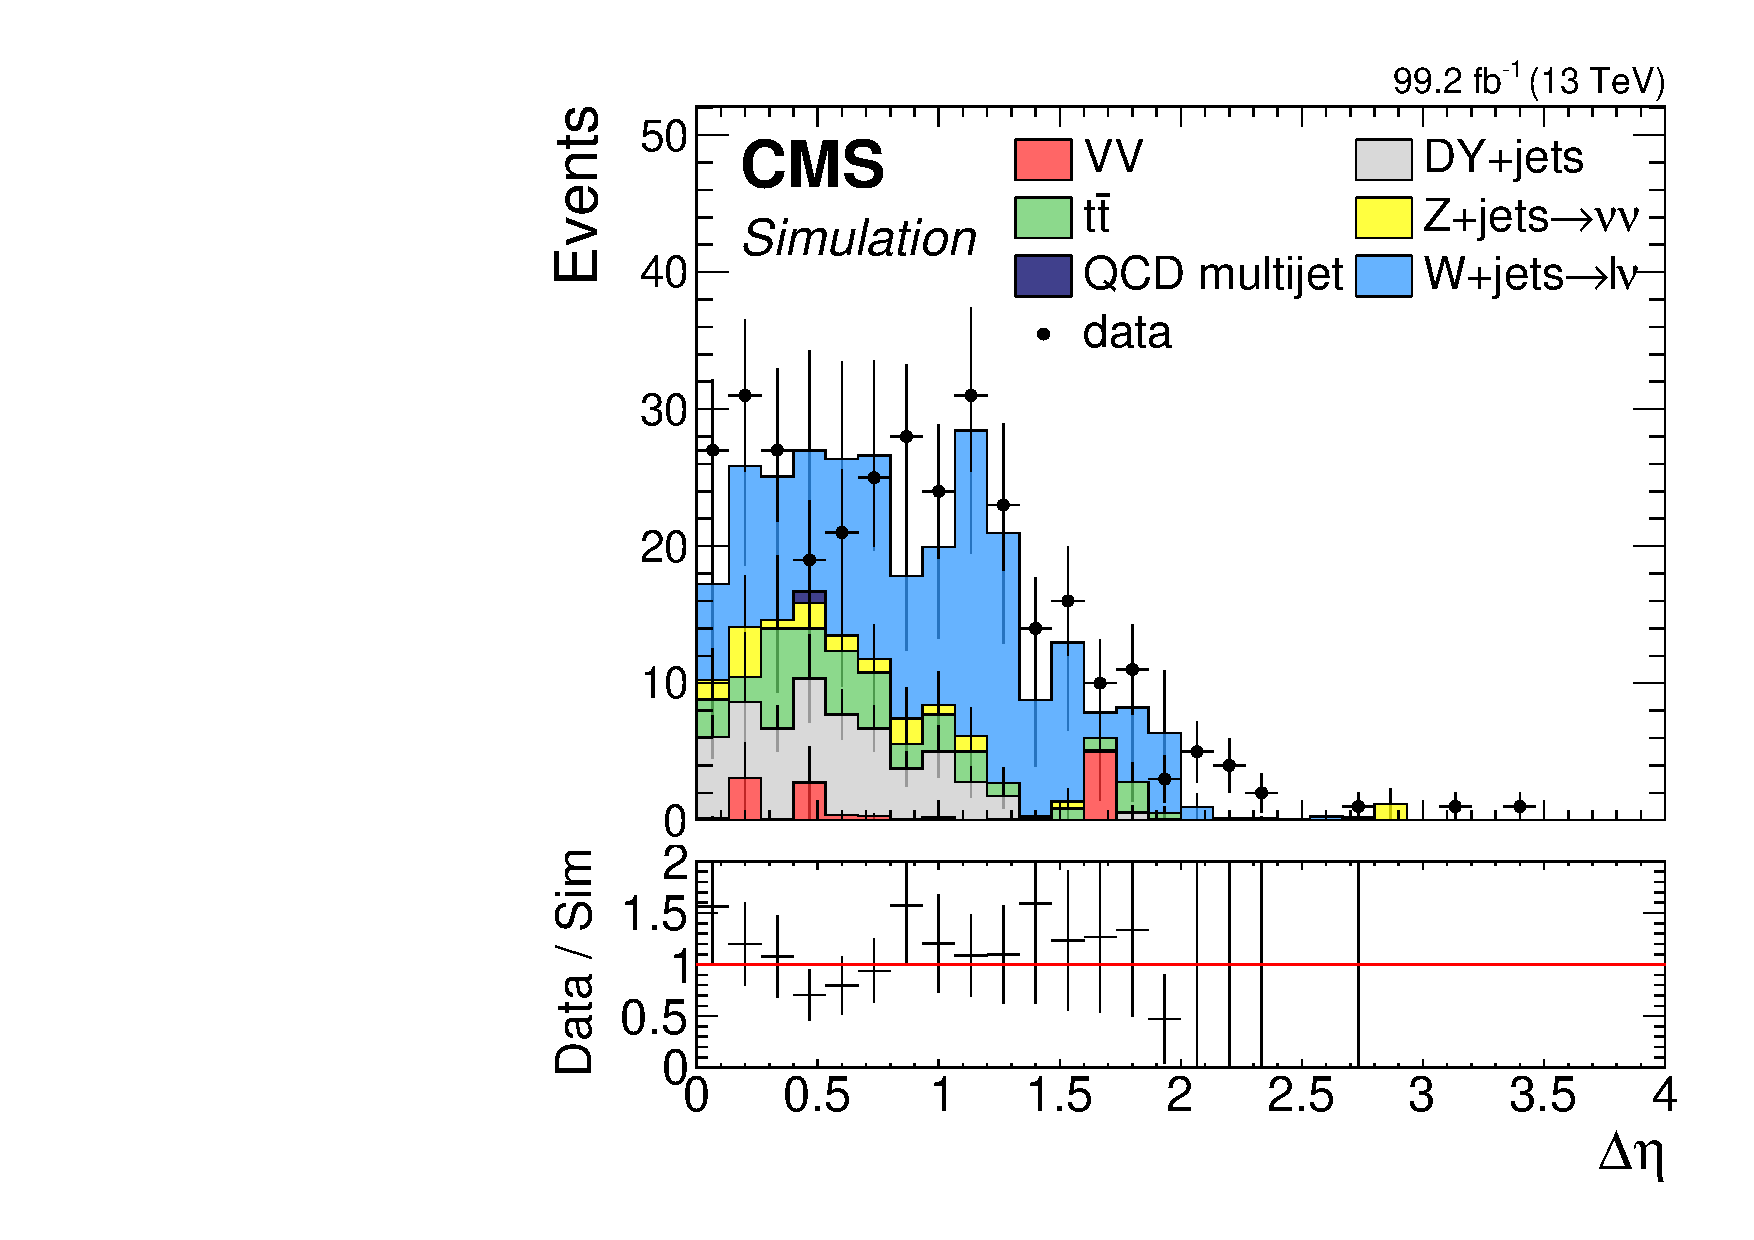
\includegraphics[width=0.48\linewidth]{plots/dilepton_muons_data_control_region_phase1/none_deltaEtaCorrJetNoMultIso10Dr0.6.pdf} \,
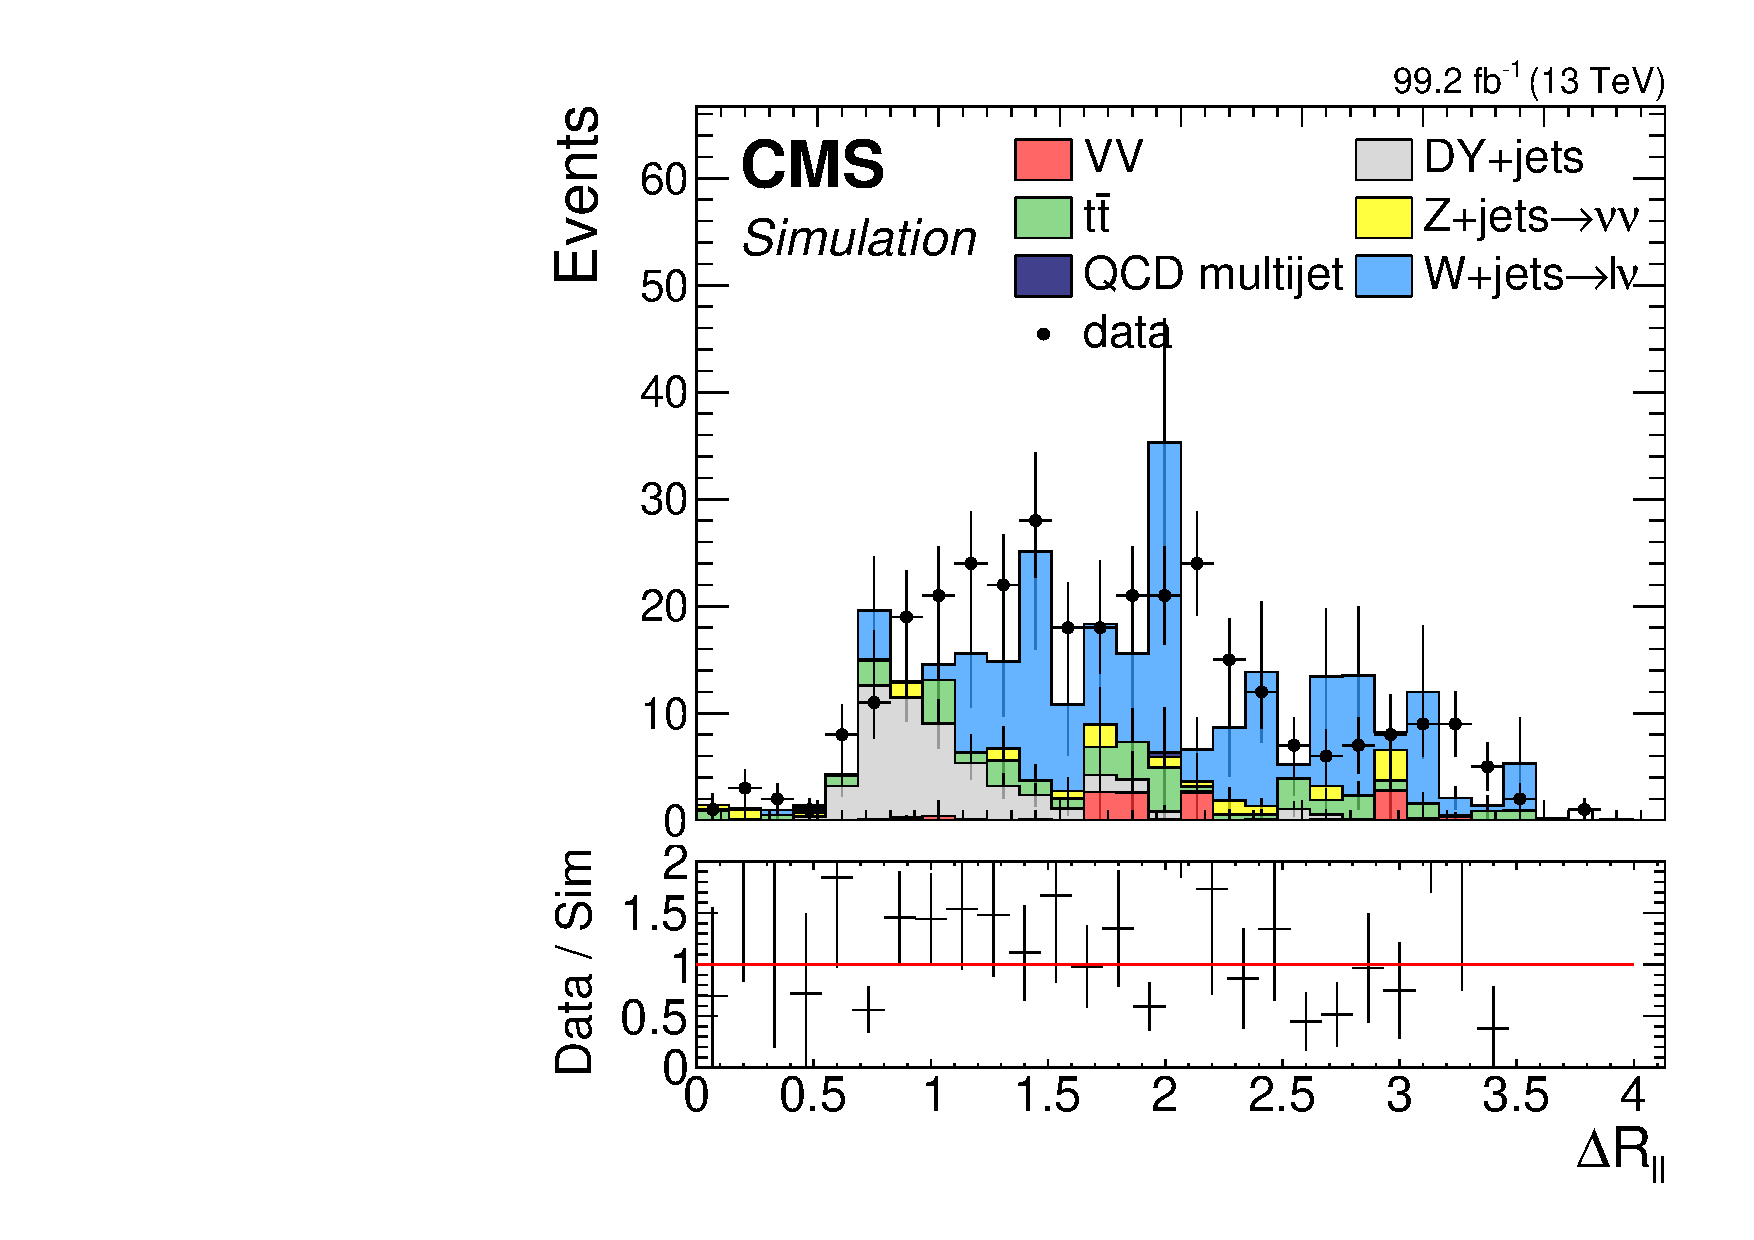
\includegraphics[width=0.48\linewidth]{plots/dilepton_muons_data_control_region_phase1/none_deltaRCorrJetNoMultIso10Dr0.6.pdf} \\

\end{figure} 